\documentclass[openany]{book}

\usepackage[margin=1in]{geometry}
\usepackage{amsmath,amsfonts,amsthm, amssymb}
\usepackage{yhmath}
\usepackage{mathrsfs}
\usepackage{mathtools}
\usepackage{xcolor}
\usepackage{graphicx}
\usepackage{comment}
\usepackage{tikz-cd}
\usepackage{quiver}
\renewcommand{\familydefault}{ppl}
\newcommand{\R}{\mathbb{R}}
\newcommand{\E}{\mathbb{E}}
\newcommand{\Z}{\mathbb{Z}}
\newcommand{\CC}{\mathcal{C}}
\newcommand{\F}{\mathbb{F}}
\newcommand{\la}{\langle}
\newcommand{\ra}{\rangle}
\newcommand{\colim}{\text{colim}}
\DeclareMathOperator{\im}{im}
\let\oldemptyset\emptyset
\let\emptyset\varnothing
\newcommand{\tor}{\text{Tor}}
\newcommand{\id}{\text{id}}
\newcommand{\ext}{\text{Ext}}
\newcommand{\ptop}{\text{PTop}}
\newcommand{\pt}{\text{pt}}
\newcommand{\ach}{\text{Ach}}


\usepackage{thmtools,thm-restate}

% Fixing mdframed skip below
% See https://tex.stackexchange.com/a/292090/143086
\usepackage[framemethod=TikZ]{mdframed}
\usepackage{xpatch}
\makeatletter
\xpatchcmd{\endmdframed}
	{\aftergroup\endmdf@trivlist\color@endgroup}
	{\endmdf@trivlist\color@endgroup\@doendpe}
	{}{}
\makeatother

\definecolor{huilightpink}{HTML}{fff2fe}
\definecolor{huidarkpink}{HTML}{d955b7}
\declaretheoremstyle[
	mdframed={
		backgroundcolor=huilightpink,
		linecolor=huidarkpink,
		rightline=false,
		topline=false,
		bottomline=false,
		linewidth=2pt,
		innertopmargin=5pt,
		innerbottommargin=8pt,
		innerleftmargin=8pt,
		leftmargin=-2pt,
		skipbelow=2pt,
		nobreak
	},
	headfont=\normalfont\bfseries\color{huidarkpink}
]{huipinkbox}
\declaretheorem[style=huipinkbox,name=Theorem,within=chapter]{thm}
\declaretheorem[style=huipinkbox,name=Theorem,sibling=thm]{theorem}




\begin{comment}
\definecolor{huilightyellow}{HTML}{fff5d6}
\definecolor{huidarkyellow}{HTML}{fcad03}
\declaretheoremstyle[
	mdframed={
		backgroundcolor=huilightyellow,
		linecolor=huidarkyellow,
		rightline=false,
		topline=false,
		bottomline=false,
		linewidth=2pt,
		innertopmargin=5pt,
		innerbottommargin=8pt,
		innerleftmargin=8pt,
		leftmargin=-2pt,
		skipbelow=2pt,
		nobreak
	},
	headfont=\normalfont\bfseries\color{huidarkyellow}
]{huiyellowbox}
\declaretheorem[style=huiyellowbox,name=Proposition,within=chapter]{prop}
\end{comment}



\definecolor{huilightpurple}{HTML}{faf2ff}
\definecolor{huidarkpurple}{HTML}{912ed9}
\declaretheoremstyle[
	mdframed={
		backgroundcolor=huilightpurple,
		linecolor=huidarkpurple,
		rightline=false,
		topline=false,
		bottomline=false,
		linewidth=2pt,
		innertopmargin=5pt,
		innerbottommargin=8pt,
		innerleftmargin=8pt,
		leftmargin=-2pt,
		skipbelow=2pt,
		nobreak
	},
	headfont=\normalfont\bfseries\color{huidarkpurple}
]{huipurplebox}
\declaretheorem[style=huipurplebox,name=Proposition,within=chapter]{prop}



% \definecolor{huilightpurple}{HTML}{faf2ff}
% \definecolor{huidarkpurple}{HTML}{912ed9}
% \declaretheoremstyle[
% 	mdframed={
% 		backgroundcolor=huilightpurple,
% 		linecolor=huidarkpurple,
% 		rightline=false,
% 		topline=false,
% 		bottomline=false,
% 		linewidth=2pt,
% 		innertopmargin=5pt,
% 		innerbottommargin=8pt,
% 		innerleftmargin=8pt,
% 		leftmargin=-2pt,
% 		skipbelow=2pt,
% 		nobreak
% 	},
% 	headfont=\normalfont\bfseries\color{huidarkpurple}
% ]{huipurplebox}
\declaretheorem[style=huipurplebox,name=Lemma,within=chapter]{lem}


\definecolor{lightpink}{HTML}{f0f6fc}
\definecolor{darkpink}{HTML}{2c72b8}
\declaretheoremstyle[
	mdframed={
		backgroundcolor=lightpink,
		linecolor=darkpink,
		rightline=false,
		topline=false,
		bottomline=false,
		linewidth=2pt,
		innertopmargin=5pt,
		innerbottommargin=8pt,
		innerleftmargin=8pt,
		leftmargin=-2pt,
		skipbelow=2pt,
		nobreak
	},
	headfont=\normalfont\bfseries\color{darkpink}
]{pinkbox}
\declaretheorem[style=pinkbox,name=Definition,within=chapter]{defn}


\definecolor{huilightblue}{HTML}{edf9ff}
\definecolor{huidarkblue}{HTML}{4b79db}
\declaretheoremstyle[
	mdframed={
		backgroundcolor=huilightblue,
		linecolor=huidarkblue,
		rightline=false,
		topline=false,
		bottomline=false,
		linewidth=2pt,
		innertopmargin=5pt,
		innerbottommargin=8pt,
		innerleftmargin=8pt,
		leftmargin=-2pt,
		skipbelow=2pt,
		nobreak
	},
	headfont=\normalfont\bfseries\color{huidarkblue}
]{huiblueblox}
\declaretheorem[style=huiblueblox,name=Example,within=chapter]{example}



% \definecolor{huilightblue}{HTML}{edf9ff}
% \definecolor{huidarkblue}{HTML}{4b79db}
% \declaretheoremstyle[
% 	mdframed={
% 		backgroundcolor=huilightblue,
% 		linecolor=huidarkblue,
% 		rightline=false,
% 		topline=false,
% 		bottomline=false,
% 		linewidth=2pt,
% 		innertopmargin=5pt,
% 		innerbottommargin=8pt,
% 		innerleftmargin=8pt,
% 		leftmargin=-2pt,
% 		skipbelow=2pt,
% 		nobreak
% 	},
% 	headfont=\normalfont\bfseries\color{huidarkblue}
% ]{huiblueblox}
% \declaretheorem[style=huiblueblox,name=Example,within=chapter]{example}

% \declaretheoremstyle[
% 	mdframed={
% 		backgroundcolor=huilightblue,
% 		linecolor=huidarkblue,
% 		rightline=false,
% 		topline=false,
% 		bottomline=false,
% 		linewidth=2pt,
% 		innertopmargin=5pt,
% 		innerbottommargin=8pt,
% 		innerleftmargin=8pt,
% 		leftmargin=-2pt,
% 		skipbelow=2pt,
% 		nobreak
% 	},
% 	headfont=\normalfont\bfseries\color{huidarkblue}
% ]{huiblueblox}
\declaretheorem[style=huiblueblox,name=Problem,within=chapter]{prob}



% \declaretheoremstyle[
% 	mdframed={
% 		backgroundcolor=huilightblue,
% 		linecolor=huidarkblue,
% 		rightline=false,
% 		topline=false,
% 		bottomline=false,
% 		linewidth=2pt,
% 		innertopmargin=5pt,
% 		innerbottommargin=8pt,
% 		innerleftmargin=8pt,
% 		leftmargin=-2pt,
% 		skipbelow=2pt,
% 		nobreak
% 	},
% 	headfont=\normalfont\bfseries\color{huidarkblue}
% ]{huiblueblox}
\declaretheorem[style=huiblueblox,name=Exercise,within=chapter]{exer}
\declaretheorem[style=huipinkbox, name=Corollary, within=chapter]{cor}





















\newcommand{\nirwarnsymbol}{%
	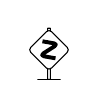
\begin{tikzpicture}[baseline=(x.base)]
		\draw[rounded corners=.01em] (-.05em,-1.07em)rectangle(.05em,.78em);
		\draw[fill=white,rounded corners=1.3] (0,.75em)--(.75em,0)--(0,-.75em)--(-.75em,0)--cycle;
		\draw[line width=0.2mm, line cap=round](-.4em,-1.07em)--(.4em,-1.07em);
		\node(x) at (0,0em) {};
		% Thank you https://tex.stackexchange.com/a/262510
		\draw[
			line cap=but,
			line join=round,
			x=.5em,
			line width=0.5mm,
			y=1*(height("Z")-\pgflinewidth)*(1-sin(10)),
			rotate=-10,
			rounded corners=1.5pt,
		](-0.57, 0.57) -- (0.57, 0.57) -- (-0.57, -0.57) -- (0.57, -0.57);
	\end{tikzpicture}%
}

%%%%%%%%%%%%%%%%%%%%%%%%%%%%%%%%%%%%%%%%%%%% MARGINS
\usepackage{marginnote}
% Thank you https://tex.stackexchange.com/a/472882
% Makes marginnotes always appear on the left, apparently
%
\makeatletter
\long\def\@mn@@@marginnote[#1]#2[#3]{%
	\begingroup
		\ifmmode\mn@strut\let\@tempa\mn@vadjust\else
			\if@inlabel\leavevmode\fi
			\ifhmode\mn@strut\let\@tempa\mn@vadjust\else\let\@tempa\mn@vlap\fi
		\fi
		\@tempa{%
			\vbox to\z@{%
				\vss
				\@mn@margintest
				\if@reversemargin\if@tempswa
						\@tempswafalse
					\else
						\@tempswatrue
				\fi\fi

					\llap{%
						\vbox to\z@{\kern\marginnotevadjust\kern #3
							\vbox to\z@{%
								\hsize\marginparwidth
								\linewidth\hsize
								\kern-\parskip
								%\mn@parboxrestore
								\marginfont\raggedleftmarginnote\strut\hspace{\z@}%
								\ignorespaces#1\endgraf
								\vss
							}%
							\vss
						}%
						\if@mn@verbose
							\PackageInfo{marginnote}{xpos seems to be \@mn@currxpos}%
						\fi
						\begingroup
							\ifx\@mn@currxpos\relax\else\ifx\@mn@currpos\@empty\else
									\kern\@mn@currxpos
							\fi\fi
							\ifx\@mn@currpage\relax
								\let\@mn@currpage\@ne
							\fi
							\if@twoside\ifodd\@mn@currpage\relax
									\kern-\oddsidemargin
								\else
									\kern-\evensidemargin
								\fi
							\else
								\kern-\oddsidemargin
							\fi
							\kern-1in
						\endgroup
						\kern\marginparsep
					}%
			}%
		}%
	\endgroup
}
\makeatother
%
% Mostly for todonotes
\renewcommand{\marginpar}{\marginnote}
%%%%%%%%%%%%%%%%%%%%%%%%%%%%%%%%%%%%%%%%%%%% /MARGINS

\definecolor{nirlightred}{RGB}{250, 220, 220}
\definecolor{nirdarkred}{HTML}{f40000}
\declaretheoremstyle[
	mdframed={
		backgroundcolor=nirlightred,
		linecolor=nirdarkred,
		rightline=false,
		topline=false,
		bottomline=false,
		linewidth=2pt,
		innertopmargin=5pt,
		innerbottommargin=8pt,
		innerleftmargin=8pt,
		leftmargin=-2pt,
		skipbelow=2pt,
		nobreak
	},
	headfont=\normalfont\bfseries\color{nirdarkred}
]{nirredbox}

% \makeatletter
% \declaretheorem[
% 	style=nirredbox,
% 	name=Warning,
% 	sibling=thm,
% 	% without \leavevmode, the first item in a list gets misformatted
% 	postheadhook={\leavevmode\marginnote{\nirwarnsymbol}[-3pt]%
% 	\ifthmt@thisistheone% restatable makes alignment weird
% 		\hspace{-2.2pt}%
% 	\fi}
% ]{warn}
% \makeatother

\newcommand{\nirideasymbol}{%
	
\begin{tikzpicture}[baseline=(x.base)]
		\draw[rounded corners=.01em] (-.05em,-1.07em)rectangle(.05em,.78em);
		\draw[fill=white,rounded corners=1.3] (0,.75em)--(.75em,0)--(0,-.75em)--(-.75em,0)--cycle;
		\draw[line width=0.2mm, line cap=round](-.4em,-1.07em)--(.4em,-1.07em);
		\node(x) at (0,0em) {};
		\node at (0,0em) {{\textbf{!}}};
	\end{tikzpicture}%
}
\renewcommand{\nirwarnsymbol}{%
	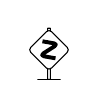
\begin{tikzpicture}[baseline=(x.base)]
		\draw[rounded corners=.01em] (-.05em,-1.07em)rectangle(.05em,.78em);
		\draw[fill=white,rounded corners=1.3] (0,.75em)--(.75em,0)--(0,-.75em)--(-.75em,0)--cycle;
		\draw[line width=0.2mm, line cap=round](-.4em,-1.07em)--(.4em,-1.07em);
		\node(x) at (0,0em) {};
		% Thank you https://tex.stackexchange.com/a/262510
		\draw[
			line cap=but,
			line join=round,
			x=.5em,
			line width=0.5mm,
			y=1*(height("Z")-\pgflinewidth)*(1-sin(10)),
			rotate=-10,
			rounded corners=1.5pt,
		](-0.57, 0.57) -- (0.57, 0.57) -- (-0.57, -0.57) -- (0.57, -0.57);
	\end{tikzpicture}%
}
\makeatletter
\declaretheorem[
	style=nirredbox,
	name=Idea,
	sibling=thm,
	% without \leavevmode, the first item in a list gets misformatted
	postheadhook={\leavevmode\marginnote{\nirideasymbol}[-3pt]%
	\ifthmt@thisistheone% restatable makes alignment weird
		\hspace{-2.2pt}%
	\fi}
]{idea}

\declaretheorem[
	style=nirredbox,
	name=Warning,
	sibling=thm,
	% without \leavevmode, the first item in a list gets misformatted
	postheadhook={\leavevmode\marginnote{\nirwarnsymbol}[-3pt]%
	\ifthmt@thisistheone% restatable makes alignment weird
		\hspace{-2.2pt}%
	\fi}
]{warn}
\makeatother

\title{Algebraic Topology}

\date{\today}
\author{Hui Sun}

\begin{document}

\maketitle

\tableofcontents



\newpage

\chapter{Category Theory}
\textbf{Instructor:} Nitu Kitchro, 
\textbf{Office Hours}: Monday after class, \textbf{TA: } Anna Matsui
\section{Lecture 1 8/26}
\begin{defn}[Category]
    A category $\mathcal{C}$ consists of the following data:
    \begin{enumerate}
        \item A collection of objects denoted as Ob$(\mathcal{C})$
        \item Given two objects $X,Y\in$ Ob$(\mathcal{C})$, a collection of morphisms between $X,Y$, $f:X\to Y$, denoted as mor$_\CC(X,Y)$.
        \item (Composition) We have mor$_\CC(X,Y)\times mor_\CC(Y,Z)\to mor_\CC(X,Z)$ that satisfies associativity
        \begin{equation*}
            f\circ(g\circ h)=(f\circ g)\circ h
        \end{equation*}
        \item (Identity) There is a distinguished morphism for each $X$, $Id_\CC(X,X)$ such that given any $f\in mor(X,Y)$, we have $f\circ id_X=id_Y\circ f=f$.
    \end{enumerate}
\end{defn}
In this course, we will make the assumption that in all the categories that we work with, Ob$(\CC)$ need not be a set, but given any $X,Y\in Ob(\CC)$, mor$(X,Y)$ will always be a set. Now we talka bout some examples of categories.
\begin{example}[Sets]
    Let Ob$(Sets)$ be all the sets in the universe. Given $X,Y$ sets, mor$(X,Y)$ be all the set maps from $X$ to $Y$, and $id_X$ is the identity map.
\end{example}
\begin{example}[Top]
    Let Ob$(Top)$ be all the topological spaces, and mor$(X,Y)$ be all the continuous maps from $X$ to $Y$.
\end{example}
\begin{example}[Vect$_\F$]
    Let $\F$ be a field, and let Ob be all the $\F$-vector spaces. Then mor$(V,W)$ is all the $\F$-linear homomorphisms from $V$ to $W$, where $id_V$ is the identity homomorphism.
\end{example}
\begin{example}[Posets]
    Fix a poset $P$, let Ob$(P)$ be the collection of elements in $P$, and given $p,q$ we define 
    \begin{equation*}
        mor(p,q)=\begin{cases}
            *, \text{ if } q\leq p\\
            \emptyset, \text{ otherwise }
        \end{cases}
    \end{equation*}
\end{example}
\begin{prob}
    \textbf{HW(Q1): check this is a category}
\end{prob}
\begin{example}[Opposite category]
    Given a category $\CC$, there is another category called the opposite category, denoted as $\CC^{op}$, where 
    \begin{enumerate}
        \item The objects are the same as $\CC$
        \item Given $X,Y\in$ Ob$(C^{op})$, we have mor$_{op}(X,Y):=$ mor$_\CC(Y,X)$. 
        \item Moreover, given $f\in mor_{op}(X,Y), g\in mor_{op}(Y,Z)$, then $g\circ f$ in $C^{op}$ is $f\circ g: Z\to X$.
    \end{enumerate}
\end{example}
Naturally, we define isomorphisms now.
\begin{defn}[isomorphism]
    Given a category $\CC$, and a morphism $f\in mor_C(X,Y)$, we say $f$ is an isomorphism if there exists $g\in mor_C(Y,X)$ such that 
    \begin{equation*}
        f\circ g=Id_Y, g\circ f=Id_X
    \end{equation*}
\end{defn}
Now we introduce maps between categories.
\begin{defn}[functor]
    Given categories $\CC,\mathcal{D}$, a functor $F:C\to D$ is the following;
    \begin{enumerate}
        \item Given an object $X$ in $\mathcal{C}$, $F(X)$ is an object in $D$. 
        \item Given a morphism $f: X\to Y$, $F(f)$ is a functor $F(f): F(X)\to F(Y)$. Moreover, it satisfies the following:
        \begin{enumerate}
            \item $F(id_X)=id_{F(X)}$
            \item $F(f\circ g)=F(f)\circ F(g)$. Alternatively, we can rewrite this condition as the following: 
            \[\begin{tikzcd}
                {mor(X,Y)\times mor(Y,Z)} & {mor(X,Z)} \\
                {mor(F(X), F(Y))\times mor(F(Y),F(Z))} & {mor(F(X),F(Z))}
                \arrow[from=1-1, to=1-2]
                \arrow["{mor(F)\times mor(F)}", from=1-1, to=2-1]
                \arrow["{mor(F)}", from=1-2, to=2-2]
                \arrow[from=2-1, to=2-2]
            \end{tikzcd}\]
            such that this diagram commutes.
        \end{enumerate}
    \end{enumerate}
\end{defn}
\begin{prob}
    \textbf{HW(Q2): functors take isomorphisms to isomorphisms.}
\end{prob}
Now we talk about some examples of functors.
\begin{example}
    $F: Top\to Set$, where $X\mapsto X$, where the latter is a set, and $f\mapsto f$ as set maps.
\end{example}
\begin{example}
    Let $\F$ be a field, and $F: Sets\to \text{Vect}_\F$, where $X\mapsto \F\la X\ra$, where $\F\la X\ra$ is the free vector space over $\F$ on the set $X$.
\end{example}
\begin{prob}
    \textbf{HW(Q3): extend this to a functor by defining $mor(f)$ and show this is a functor.}
\end{prob}
\begin{example}
    Let $\F$ be a field, then the following is a functor, $F: Sets^{op}\to\text{Vect}_\F$, where
    \begin{equation*}
        h  F: X\mapsto Maps(X,\F)
    \end{equation*}
\end{example}
\begin{prob}
    \textbf{HW(Q4)}: show this extends to a functor by defining $F(f)$, and show it is a functor.
\end{prob}

\section{Lecture 2 8/28}
\begin{defn}[contravariant functor]
    Let $F:\CC\to\mathcal{D}$ is a contravariant functor from $\CC^{op}\to\mathcal{D}$, (equivalently, $\CC\to\mathcal{D}^{op}$).
\end{defn}
\begin{prob}
    \textbf{HW(Q5):} Show that the following functor $F$ from Vect$_\F$ to Vect$_\F$ extends to a contravariant functor, where 
    \begin{equation*}
        Ob_F: V\mapsto V^*=Hom(V,\F)
    \end{equation*}
    i.e., define the morphism function and show it is a contravariant functor.
\end{prob}
We remark that we can define a category of categories: let $Cat$ be the category of categories, with morphisms as functors, and note that objects or morphisms in this case are both not sets!
\begin{defn}[natural transformation]
    Given functors $F,G: \CC\to\mathcal{D}$, a natural transformation $T$ from $F$ to $G$ is the following: $T: F\Rightarrow G$:
    \begin{enumerate}
        \item given object $X\in Ob(\CC)$, $T(X)\in mor(F(X),G(X))$
        \item Given $f\in mor(X,Y)$, the following diagram commutes:
        \[\begin{tikzcd}
            {F(X)} & {F(Y)} \\
            {G(X)} & {G(Y)}
            \arrow["{F(f)}", from=1-1, to=1-2]
            \arrow["{T(X)}"', from=1-1, to=2-1]
            \arrow["{T(Y)}", from=1-2, to=2-2]
            \arrow["{G(f)}"', from=2-1, to=2-2]
        \end{tikzcd}\]
        where $mor_F, mor_G$ is the identification function on morphisms by functors $F,G$
    \end{enumerate}
    If for all $X$, $T(X)$ is an isomorphism, then this natural transformation is called a natural isomorphism.
\end{defn}
In other words, this natural transformation is how one takes a functor $F$ and turn it to another functor $G$. We will (in a homework) show there exists natural transofrmation between the following two functors.
\begin{example}
    Consider $F,G: Vect_\F\to Vect_\F$, define 
    \begin{equation*}
        F(V)=V\otimes_\F V/_{\la a\otimes b-b\otimes a\ra}=V\otimes_\F V/\Sigma_2, G(V)=(V\otimes_F V)^{\Sigma_2}=\{\alpha\in V\otimes_\F V: \sigma(\alpha)=\alpha\}
    \end{equation*}
    Both are vector spaces are fixed under ``swaps.'' Then a natural transformation can be defined as follows $T(V):$
    \begin{equation*}
        T(V): a\otimes b\mapsto a\otimes b+b\otimes a
    \end{equation*}
\end{example}
\begin{prob}
    \textbf{HW(Q6):} For the above $F,G$
    \begin{enumerate}
        \item Show that $T$ defines a natural transformation from $F$ to $G$. 
        \item Find conditions on $\F$ for $T$ being a natural isomorphism.
    \end{enumerate}
\end{prob}
Next we define limits and colimits.
    Let $\mathcal{C},\mathcal{D}$ be categories, $d$ be an object in $\mathcal{D}$, then we can define a functor $F_d: \mathcal{C}\to\mathcal{D}$ such that for any object $c$ in $\mathcal{C}$,
    \begin{equation*}
        F_d(c)=d, F_d(f)=Id_d
    \end{equation*}
    In other words, this is the ``constant functor'' on $\mathcal{D}$, i.e., every object is sent to $d$, and every morphism is sent to $id_d$.
\begin{defn}[colimit]
    Given any functor $F:\mathcal{C}\to\mathcal{D}$, the colimit of $F$, denoted as $\colim(F)$ is an object in $\mathcal{D}$ endowed with a natural transformation:
    \begin{equation*}
        \varphi_F:F\Rightarrow F_{\colim(F)}
    \end{equation*}
    such that given any other object $d$ in $D$ and a natural transformation 
    \begin{equation*}
        \varphi: F\Rightarrow F_d
    \end{equation*}
    there exists a unique morphism in $\mathcal{D}$, $f:\colim(F)\to d$ making the following diagram commute: for any $X,Y,g$:
    \[\begin{tikzcd}
        {F(X)} && {F(Y)} \\
        & {\text{colim}(F)} \\
        & d
        \arrow["{F(g)}", from=1-1, to=1-3]
        \arrow["{\varphi_F}", from=1-1, to=2-2]
        \arrow["\varphi"', curve={height=12pt}, from=1-1, to=3-2]
        \arrow["{\varphi_F}"', from=1-3, to=2-2]
        \arrow["\varphi", curve={height=-12pt}, from=1-3, to=3-2]
        \arrow["{\textcolor{red}{f}}", from=2-2, to=3-2]
    \end{tikzcd}\]
\end{defn}
Next we prove some facts about colimits and give an example, where $\colim(F)$ exists.
\begin{prop}
    If $\colim F$ exists, then $\colim F$ is unique up to isomorphisms.
\end{prop}
\begin{proof}
    Let $\colim(F), \colim(F)'$ be two colimits that satisfy the criteria. They are both objects in $\mathcal{D}$, then we get a morphism $f:\colim(F)\to\colim(F)'$, and likewise $g:\colim(F)\to\colim(G)'$, then
    \begin{equation*}
        f\circ g:\colim(F)'\to\colim(F)'
    \end{equation*} 
    is the only morphism, and is the identity morphism. Similarly for $g\circ f$.
\end{proof}
Next we demonstrate a fact via an example.
\begin{thm}
    Let $\mathcal{C}$ be a category where $Ob(\mathcal{C}), mor(X,Y)$ are all sets. Let $F: \mathcal{C}\to\text{Top}$ be any functor, then $\colim(F)$ exists.
\end{thm}
\begin{proof}
    Define $\colim(F):=\bigsqcup_{c}F(c)/\sim$, where $\sim$ is induced by the equivalence relation given by 
    \begin{equation*}
        y\sim F(f)y
    \end{equation*}
    where $y\in F(C_1), f:C_1\to C_2, F(f)x\in F(C_2)$. The natural transformation we endow on $F$ as $\varphi_F:F\Rightarrow F_{\colim(F)}$:
    \begin{equation*}
        \varphi_F: F(C)\mapsto \bigsqcup_{C\in Ob(C)}F(C)/\sim
    \end{equation*}
\end{proof}
\begin{prob}
    \textbf{HW(Q7):} Show that $\colim(F), \varphi_F$ is indeed a colimit. 
\end{prob}
We note that colimits also exist (the same argument goes through) if we replace $\text{Top}$ with groups, sets, but with slightly different constructions, replacing disjoint unions with products, etc.

\begin{defn}[limit]
    Given a functor $F: \mathcal{C}\to\mathcal{D}$, the limit of $F$, denoted as $\lim(F)$ is an object of $\mathcal{D}$, endowed with a natural transformation:
    \begin{equation*}
        \varphi_F: F_{\lim(F)}\Rightarrow F
    \end{equation*}
    such that given any other object $d\in Ob(\mathcal{D})$ and a natural transformation 
    \begin{equation*}
        \varphi: F_d\to F
    \end{equation*}
    there exists a unique $f: \lim F\to d$ such that the following diagram commutes:
    \[\begin{tikzcd}
        & {\lim F} \\
        & d \\
        {F(X)} && {F(Y)}
        \arrow["{\textcolor{red}{f}}", from=1-2, to=2-2]
        \arrow["{\varphi_F}"', curve={height=12pt}, from=1-2, to=3-1]
        \arrow["{\varphi_F}"', curve={height=-12pt}, from=1-2, to=3-3]
        \arrow["\varphi"', from=2-2, to=3-1]
        \arrow["\varphi", from=2-2, to=3-3]
        \arrow["{F(g)}"', from=3-1, to=3-3]
    \end{tikzcd}\]
\end{defn}
Just like colimits, limits are unique up to isomorphisms. 
\begin{prob}
    \textbf{HW(Q8):} Given $F:\mathcal{C}\to\mathcal{D}$, consider $F^{op}:\mathcal{C}^{op}\to\mathcal{D}^{op}$, then 
    \begin{equation*}
        \lim F=\colim F^{op}
    \end{equation*}
\end{prob}
The above problem is interpretation of diagrams and essentially we just reverse all the maps.

\section{Lecture 3 9/4}
Today we define (co)chain complexes: let $R$ be a commutative ring, let $Mod_R$ denote the category of $R$-modules and $R$-module maps.
\begin{defn}[chain complex]
    A chain complex of $R$-modules is a collection of $R$-modules and $R$-modules maps 
    \begin{equation*}
        \dots\to M_{i+1}\xrightarrow{\partial_{i+1}}M_i\xrightarrow{\partial_i}M_{i-1}\xrightarrow{\partial_{i-1}}\dots
    \end{equation*}
    such that $\partial_i\circ\partial_{i+1}=0$ for all $i$. In other words, the image of previous map is contained in the kernal of the subsequent map. In short, we have 
    \begin{equation*}
        \partial^2=0
    \end{equation*}
    We will denote a chain complex by $\{M.; \partial.^M\}$.
\end{defn}
Next we introduce morphisms between chain complexes.
\begin{defn}[morphism between complexes]
    Let $\{M.;\partial.^M\}, \{N.;\partial.^N\}$, a morphism $\{f.\}$ between chain complexes is a ``ladder'' such that the following commutes:
    \[\begin{tikzcd}
        \dots & {M_{i+1}} & {M_i} & {M_{i-1}} & \dots \\
        \dots & {N_{i+1}} & {N_i} & {N_{i-1}} & \dots
        \arrow[from=1-1, to=1-2]
        \arrow["{\partial_{i+1}^M}", from=1-2, to=1-3]
        \arrow["{\partial_i^M}", from=1-3, to=1-4]
        \arrow[from=1-4, to=1-5]
        \arrow[from=2-1, to=2-2]
        \arrow["{\partial_{i+1}^N}", from=2-2, to=2-3]
        \arrow["{\partial_{i}^N}", from=2-3, to=2-4]
        \arrow[from=2-4, to=2-5]
    \end{tikzcd}\]
    Moreover, we define composition of morphisms:
    \begin{equation*}
        \{f.\}\circ \{g.\}:=\{(f\circ g).\}
    \end{equation*}
    where $\{g.\}:\{M.;\partial.^M\}\to\{N.;\partial.^N\}$, and $\{f.\}:\{N.;\partial.^N\}\to \{L.;\partial.^L\}$, which is simply vertical stacking.
\end{defn}
\begin{prob}
    \textbf{HW(Q9):} Prove that chain complexes of $R$-modules form a category $\text{ch}_R$.
\end{prob}
There are interesting functors $F:\text{ch}_R\to Mod_R$, and we begin with the following one:
\begin{defn}[$H_n$, $n$th-homology]
    Given $n\in\mathbb{Z}$, there is a functor 
    \begin{equation*}
        H_n: \text{ch}_R\to Mod_R
    \end{equation*}
    defined as follows:
    \begin{equation*}
        H_n(\{M.;\partial.^M\}):=\ker\partial_n^M\big/ Im \partial_{n+1}^M
    \end{equation*}
    and for $f:\{M.;\partial.^M\}\to\{N.;\partial.^N\}$, we define: $H_n(f): H_n(\{M.;\partial.^M\})\to H_n(\{N.;\partial.^N\})$,
    \begin{equation*}
        H_n(f)[x]:=[f_n(x)]
    \end{equation*}
    where $[x]\in H_n(\{M.;\partial.^M\})$.
\end{defn}


\section{Lecture 10/09}

Last time we showed that 
\begin{equation*}
    S_\bullet(X,R)\otimes_R S_\bullet(Y,R) \text{ and } S_\bullet(X\times Y,R)
\end{equation*}
are chain homotopic. We now make a few remarks:
\begin{enumerate}
    \item The above theorem extends to a relative natrual equivalence: using naturality of the non-relative theorem: $EZ: S_\bullet(X,A,R)\otimes S_\bullet(Y,B,R)\to S_\bullet(X\times Y, X\times B\cup A\times Y, R)$
    \item On the level of cochain cmplexes, we have corresponding cochain homotpy equivalences: 
    \begin{equation*}
        EZ^*: S^\bullet(X\times Y, R)to S^\bullet(X,R)\otimes S^\bullet(Y,R)
    \end{equation*}
    and more generally for relative equivalences.
    \item If $X=Y$, then there is a nice classification of the following composite:
    \[\begin{tikzcd}
        {S_\bullet(X,R)} & {S_\bullet(X\times X,R)} & {S_\bullet(X,R)\otimes S_\bullet(X,R)}
        \arrow["{\Delta_*}", from=1-1, to=1-2]
        \arrow["{EZ^{-1}}", from=1-2, to=1-3]
    \end{tikzcd}\]
    given by the Alexander-Whitney diagonal formula, where $\Delta_*$is the map induced by the diagonal map:
    \begin{equation*}
        \Delta:X\to X\times X
    \end{equation*}
    where $x\mapsto (x,x)$.
\end{enumerate}
Next we talk about the Alexander-Whiteney construction.
\begin{defn}
    The Alexander-Whiteney diagonal is a natural map:
    \begin{equation*}
        AW: S_\bullet(X,R)\to S_\bullet(X,R)\otimes_R S_\bullet(X,R)
    \end{equation*}
    such that 
    \begin{equation*}
        AW\la f\ra=\bigoplus_{p+q=n}\la f\circ Fr^p\ra\otimes \la f\circ Bk^q\ra
    \end{equation*}
    where $Fr,Bk$ means front and back, and $f:\Delta_n\to X$ is a continuous map and 
    \begin{equation*}
        f\circ Fr^p
    \end{equation*}
    denotes the restriction of $f$ to the front $p$-face given by 
    \begin{equation*}
        Fr^p=\{x=(t_0,\dots, t_n):t_i=0, \forall i>p\}
    \end{equation*}
    and the back $q$-face is 
    \begin{equation*}
        Bk^q=\{x=(t_0,\dots, t_n): t_i=0, \forall i<n-q\}
    \end{equation*}
\end{defn}
Note that 
\begin{equation*}
    \la f\circ Fr^p\ra\in S_p(X,R)
\end{equation*}
and 
\begin{equation*}
    \la f\circ Bk^q\ra\in S_q(X,R)
\end{equation*}
\begin{prob}[HW(3.3)]
    Show that $AW\la f\ra$ is a chain map, i.e., it commutes with the differential on both sides.
\end{prob}
\begin{thm}
    The Alexander-Whitney diagonal is naturally homotopic to the following composite:
    \[\begin{tikzcd}
        {S_\bullet(X,R)} & {S_\bullet(X\times X,R)} & {S_\bullet(X,R)\otimes S_\bullet(X,R)}
        \arrow["{\Delta_*}", from=1-1, to=1-2]
        \arrow["{EZ^{-1}}", from=1-2, to=1-3]
    \end{tikzcd}\]
\end{thm}
\begin{proof}
    Consider the functors:
    \begin{equation*}
        g,g':Top\to\ach_R
    \end{equation*}
    given by 
    \begin{equation*}
        g(X)=S_\bullet(X,R), g'(X)=S_\bullet(X,R)\otimes S_\bullet(X,R)
    \end{equation*}
    consider the collection 
    \begin{equation*}
        M=\bigsqcup_k M_k, M_k=\{\Delta_k\}
    \end{equation*}
    and let $i_k\in S_k(\Delta_k,R)$ be $\la id_{\Delta_k}\ra$. Then notice that $g$ is free with respect to $M$ and $g'$ is acyclic with respect to $M$ by the algebraic Kunneth theorem. Hence the second part of the AMT syas that the two natrual transformations $AW$ and $EZ^{-1}\circ\Delta_*$ are naturally chain homotopic.
\end{proof}
Next we prove the ES axiom 2.
\begin{prop}
    Singular homology satisfies the homotopy axiom.
\end{prop}
\begin{proof}
    \textcolor{red}{fill in later}
\end{proof} 
Next we will prove the ES A3, the Excision axiom. We introduce a few definitions before doing so. We will talk about barycentric subdivision.

\begin{defn}[barycenter]
    Let $\Delta_n$ denote the $n$-simplex, let
    \begin{equation*}
        \{e_{i_0},\dots, e_{i_k}\}
    \end{equation*}
    be some collection of vertices of $\Delta_n$. where 
    \begin{equation*}
        I=\{i_0,\dots,i_k\}\subset\{0,\dots, n\}
    \end{equation*}
    The barycenter of $I$ is 
    \begin{equation*}
        b(I)=\frac{1}{k+1}\sum_{i\in I}e_i\in \Delta_n
    \end{equation*}
    Namely, $b(I)$ is the center of the face spanned by vertices $e_i$ where $i\in I$.
\end{defn}
Let $\sigma\in S_{n+1}$ be a permutation of $\{0,\dots, n\}$. Define an $n$-simplex $B(\sigma)$ to be the subspace of $\Delta_n$ with vertices:
\begin{equation*}
    \{b(\sigma\{0,\dots,n\}), b(\sigma\{1,\dots,n\}), \dots, b(\sigma\{n\})\}
\end{equation*}
note that $b$ does not change under permuattions, i.e., 
\begin{equation*}
    B(\sigma)=\left\{\sum_{j=0}^nt_jb(\sigma\{j,\dots,n\}):t_j\geq 0, \sum_jt_j=1\right\}
\end{equation*}
\begin{defn}
    The barycentric subdivision is a natural transformation 
    \begin{equation*}
        L: S_\bullet(X)\to S_\bullet(X)
    \end{equation*}
    such that given $\la f\ra\in S_n(X)$, we define 
    \begin{equation*}
        L(\la f\ra)=\sum_{\sigma\in S_{n+1}}(-1)^{sgn(\sigma)}\la f\circ B(\sigma)\ra
    \end{equation*}
\end{defn}
\begin{prob}[HW(3.4)]
    Show that $L$ is a chain map, i.e., 
    \begin{equation*}
        \partial L=L\partial
    \end{equation*}
    Hint: in $\partial L$ the internal faces cancel off.
\end{prob}
\begin{cor}
    By AMT, we have $L^1, L^2,\dots, L^k$ areall chain homotopic to the identity transformation.
\end{cor}

We make the remark that by the naturality of $L$, we see that $L$ extends to a natural transformation
\begin{equation*}
    L: S_\bullet(X,A,R)\to S_\bullet(X,A,R)
\end{equation*}
such that $L^k$ is chain homotopic to the identity for all $k\in\mathbb{N}$.

Next time, we will talk about the Excision Axiom A3.

\section{Lecture 10/14}
We start the proof of Excision Axiom.
\begin{defn}[good cover]
    A good cover $\{U_i\}$ of a topological space $X$ is a cover such that $\{int(U_i)\}$ is an open cover of $X$. 
\end{defn}
We define chain complex 
\begin{equation*}
    \{S_\bullet^U(X,R),\partial_\bullet\}
\end{equation*}
by 
\begin{equation*}
    S_n^U(X,R)=\bigoplus_{f\in\Delta_n^U(X)}R\la f\ra
\end{equation*}
where $\Delta_n^U(X)$ is the set of all continuous maps from $\Delta_n$ to $X$ that land in some $U_i$, and the differential is given by the usual formula.

The relative version is as follows: if $A\subset X$ then $\{A\cap U_i\}$ is a good cover of $A$, which we also denote by $U$. Define 
\begin{equation*}
    S_\bullet^U(X,A,R)=\left\{S_\bullet^U(X,R)/S_\bullet^U(A,R);\partial_\bullet\right\}
\end{equation*}
is the relative version of the defintion.
\begin{prop}
    The canonical inclusion 
    \begin{equation*}
        i: S_\bullet^U(X,A,R)\to S_\bullet(X,A,R)
    \end{equation*}
    induces an isomorphism in homology:
    \begin{equation*}
        i_*: H_*(S_\bullet^U(X,A,R))\cong H_*(X,A,R)
    \end{equation*}
\end{prop}
\begin{proof}
    First we reduce to the case where $A=\emptyset$ using the 5-lemma. Consider the laddder of LES:
    \[\begin{tikzcd}
        \dots & {H_n(S_\bullet^U(A,R))} & {H_n(S_\bullet^U(X,R))} & {H_n(S^U(X,A,R))} & \dots \\
        \dots & {H_n(A,R)} & {H_n(X,R)} & {H_n(X,A,R)} & \dots
        \arrow[from=1-1, to=1-2]
        \arrow[from=1-2, to=1-3]
        \arrow["{i_A}", from=1-2, to=2-2]
        \arrow[from=1-3, to=1-4]
        \arrow["{i_X}", from=1-3, to=2-3]
        \arrow[from=1-4, to=1-5]
        \arrow["{i_{(X,A)}}", from=1-4, to=2-4]
        \arrow[from=2-1, to=2-2]
        \arrow[from=2-2, to=2-3]
        \arrow[from=2-3, to=2-4]
        \arrow[from=2-4, to=2-5]
    \end{tikzcd}\]
    So if we show that $i_A, i_X$ are isomorphisms, then $i_{(X,A)}$ is also an isomorphism by the 5-lemma. So we consider 
    \begin{equation*}
        i_*: H_*(S_\bullet^U(X,R))\to H_*(X,R)
    \end{equation*}
    First we show that $i_*$ is injective, consider 
    \[\begin{tikzcd}
        {S_{n+1}^U(X)} & {\textcolor{blue}{\beta}\in S_{n+1}(X)} \\
        {S_n^U(X)} & {\textcolor{blue}{\partial\beta}\in S_n(X)}
        \arrow["i", from=1-1, to=1-2]
        \arrow["\partial", from=1-1, to=2-1]
        \arrow["\partial", from=1-2, to=2-2]
        \arrow["i", from=2-1, to=2-2]
    \end{tikzcd}\]
    Let $[\alpha]\in H_n(S_\bullet^U(X))$ such that $i_*[\alpha]=0$. Then 
    \begin{equation*}
        \alpha=\partial\beta
    \end{equation*}
    for some $\beta\in S_{n+1}(X)$. Now apply $L^k$ for some $k>>0$. Then 
    \begin{equation*}
        L^k(\beta)\in S_{n+1}^U(X)
    \end{equation*}
    We know that 
    \begin{equation*}
        L^k(\beta)-\beta=(D\partial+\partial D)(\beta)
    \end{equation*}
    for some natural homotopy $D$, i.e., 
    \begin{align*}
        L^k(\beta)-\beta&=D\partial(\beta)+\partial D(\beta)\\
        &=D(\alpha)+\partial D(\beta)
    \end{align*}
    Hence $\beta=L^k(\beta)-\partial D(\beta)-D(\alpha)$, hence 
    \begin{equation*}
        \partial\beta=\partial(L^k(\beta)-D(\alpha))=\alpha
    \end{equation*}
    but $L^k(\beta)-D(\alpha)\in S_{n+1}^U(X,R)$, by subdivision and naturality, we see that 
    \begin{equation*}
        [\alpha]=0
    \end{equation*}
    in $H_n(S_\bullet^U(X,R))$. 
    
    Next we show that $i_*$ is surjective. Given $[\alpha]\in H_n(X,R)$, replace $[\alpha]$ with $[L^k(\alpha)]$ for $k>>0$ using the fact that $L^k$ is chain homotopic to the identity, but 
    \begin{equation*}
        L^k(\alpha)\in S_n^U(X,R)
    \end{equation*}
    so $i_*$ is surjective.
\end{proof}
\begin{cor}
    Singular homology satisfies Excision Axiom A3.
\end{cor}
\begin{proof}
    \textcolor{red}{fill in later}
\end{proof}

\begin{thm}[Mayer-Vietoris sequence]
    Let $V_1,V_2$ be such that $int(V_1)\cup int(V_2)=X$, then there is a LES:
    \[\begin{tikzcd}
        \dots & {H_i(V_1\cap V_2)} & {H_i(V_1)\oplus H_i(V_2)} & {H_i(X)} \\
        & {H_{i-1}(V_1\cap V_2)} & {H_{i-1}(V_1)\oplus H_{i-1}(V_2)} & {H_{i-1}(X)} \\
        & \dots
        \arrow[from=1-1, to=1-2]
        \arrow["s", from=1-2, to=1-3]
        \arrow["t", from=1-3, to=1-4]
        \arrow[curve={height=-6pt}, from=1-4, to=2-2]
        \arrow[curve={height=-6pt}, from=2-4, to=3-2]
    \end{tikzcd}\]
    where $s$ is induced by the map $(i_1)_*\oplus -(i_2)_*$, where 
    \begin{equation*}
        i_1:V_1\cap V_2\to V_1
    \end{equation*}
    and 
    \begin{equation*}
        i_2: V_1\cap V_2\to V_2
    \end{equation*}
    and $t$ is induced by the map 
    \begin{equation*}
        (j_1)_*+(j_2)_*
    \end{equation*}
    where 
    \begin{equation*}
        j_1:V_1\to X, j_2:V_2\to X
    \end{equation*}
\end{thm}
\begin{prob}[HW(3.5)]
    Calculate the homology of the Riemannian surface $\Sigma_g$, $g$ stands for $g$-holes. For example, $\Sigma_0=\mathbb{S}^2$, $\Sigma_1=S^1\times S^1$.
\end{prob}

Next we talk about products in cohomology. We now introduce and study 4 types of natural pairings.
\begin{enumerate}
    \item Topological crossproduct in homology:
    \begin{equation*}
        \bigoplus_{i+j=n}H_i(X,A)\otimes_R H_j(Y,B)\xrightarrow{X_\bullet}H_n(X\times Y, A\times Y\cup X\times B)
    \end{equation*}
    \item Topological cross product in cohomology:
    \begin{equation*}
        \bigoplus_{i+j=n}H^i(X,A)\otimes_R H^j(Y,B)\xrightarrow{X_\bullet}H^n(X\times Y, A\times Y\cup X\times B)
    \end{equation*}
    \item Cup product in cohomology 
    \begin{equation*}
        \bigoplus_{i+j=n}H^i(X,A)\otimes_R H^j(X,B)\xrightarrow{\cup} H^n(X,A\cup B)
    \end{equation*}
    \item Cap product between (co)homologies:
    \begin{equation*}
        \bigoplus_{i+j=n}H^i(X,A)\otimes_R H_n(X,A\cup B)\xrightarrow{\cap} H_{n-i}(X,B)
    \end{equation*}
\end{enumerate}

We start with the first type: topological product in homology. We define the natural pairing
\begin{equation*}
    \bigoplus_{i+j=n}H_i(X,A)\otimes_R H_j(Y,B)\xrightarrow{X_\bullet}H_n(X\times Y, A\times U\cup X\times B)
\end{equation*}
as the composite:
\[\begin{tikzcd}
	{H_i(S_\bullet(X,A))\otimes H_j(S_\bullet(Y,B))} & {H_n(S_\bullet(X\times Y, X\times B\cup A\times Y))} \\
	& {H_n(S_\bullet(X,A)\otimes_R S_\bullet(Y,B))}
	\arrow["{X_\bullet}", from=1-1, to=1-2]
	\arrow["{X_{alg}}"', from=1-1, to=2-2]
	\arrow["{EZ(\cong)}"', from=2-2, to=1-2]
\end{tikzcd}\]
where $X_{alg}$ denotes the algebraic cross product:
\begin{equation*}
    X_{alg}([\alpha]\otimes[\beta]):=[\alpha\otimes\beta]
\end{equation*}
We note that $X$ can be seen as a natural transforamtion between the functors $H_i\otimes H_j$ and $H_{i+j}$ from 
\begin{equation*}
    PTop\times PTop\to R-Mod
\end{equation*}

(II) Next we talk about topological crossproduct in cohomology. To define topological cross product, we first observe that for any $R$ modules $V,W$, there is a natural map 
\begin{equation*}
    Hom(V,R)\otimes_R Hom(W,R)\xrightarrow{\lambda} Hom(V\otimes W,R)
\end{equation*}
and 
\begin{equation*}
    \lambda(\varphi\otimes\psi)(a\times b)=\varphi(a)\psi(b)
\end{equation*}
We then define 
\begin{equation*}
    \bigoplus_{i+j=n}H^i(X,A)\otimes_R H^j(Y,B)\xrightarrow{X_\bullet}H^n(X\times Y, A\times U\cup X\times B)
\end{equation*}
as the composite
\[\begin{tikzcd}
	{H^i(S^\bullet(X,A))\otimes H^j(S^\bullet(Y,B))} & {H^n(S^\bullet(X\times Y, X\times B\cup A\times Y))} \\
	{H^n(S^\bullet(X,A)\otimes S^\bullet(Y,B))} & {H^n(Hom(S_\bullet(X,A)\otimes_R S_\bullet(Y,B),R))}
	\arrow["{X^\bullet}", from=1-1, to=1-2]
	\arrow["{X_{alg}}", from=1-1, to=2-1]
	\arrow["\lambda", from=2-1, to=2-2]
	\arrow["{EZ^{-1} (\cong)}"', from=2-2, to=1-2]
\end{tikzcd}\]
Note: as before, $X$ can be seen as a natural transformation between the two obvious functors.

Recall the map 
\begin{equation*}
    \beta: H^i(X,A)\to Hom(H_i(X,A),R)
\end{equation*}
\begin{prob}[HW(3.6)]
    Show the following diagram commutes:
    \[\begin{tikzcd}
        {H^i(X,A)\otimes H^j(Y,B)} & {H^{i+j}(X\times Y, X\times B\cup A\times Y)} \\
        {Hom(H_i(X,A),R)\otimes Hom(H_j(Y,B),R)} & {Hom(H_{i+j}(X\times Y, X\times B\cup A\times Y),R)} \\
        & {Hom(H_i(X,A)\otimes_R H_j(Y,B),R)}
        \arrow["{X^\bullet}", from=1-1, to=1-2]
        \arrow["{\beta\otimes\beta}"', from=1-1, to=2-1]
        \arrow["\beta", from=1-2, to=2-2]
        \arrow["\lambda"', from=2-1, to=3-2]
        \arrow["{X_\bullet^*}", from=2-2, to=3-2]
    \end{tikzcd}\]
    where $X_\bullet^*$ denotes the dual map induced by the crossproduct in the homology.
\end{prob}


\section{Lecture 10/16}



\section{Lecture 10/21}



\section{Lecture 10/23}


\section{Lecture 10/28}
Last time, we defined the cap product, we recall the definition.
\begin{equation*}
    S\cap: S^i(X)\otimes S_n(X)\to S_{n-i}(X)
\end{equation*}
where 
\begin{equation*}
    \psi\otimes\la f\ra\mapsto \psi(\la f\circ Bk^i\ra)\la f\circ Fr^{n-1}\ra
\end{equation*}
We now prove the following proposition:
\begin{prop}
    The cap product satisfies the following:
    \begin{enumerate}
        \item $1\cap\gamma=\gamma$, where $\gamma\in H_n(X)$.
        \item If $|\alpha|=|\gamma|$, then $\varepsilon(\alpha\cap\gamma)=\beta(\alpha)(\gamma)=\la\alpha,\gamma\ra$.
        \item We have $(\alpha_1\cup\alpha_2)\cap\gamma=\alpha_1\cap(\alpha_2\cap\gamma)$.
        \item If $f:X\to Y$ is continuous, $\alpha\in H^*(Y)$, and $\gamma\in H_*(X)$, then $f_*(f^*(\alpha)\cap\gamma)=\alpha\cap f_*(\gamma)$.
        \item If $|\alpha_1|+|\alpha_2|=|\gamma|$, we have $\beta(\alpha_1\cup\alpha_2)(\gamma)=\la\alpha_1\cup\alpha_2,\gamma\ra=\la \alpha_1,\alpha_2\cap\gamma\ra$.(This immediately follows from (2),(3)).
    \end{enumerate}
\end{prop}
\begin{proof}
    For 1: we know $1\cap\gamma=\gamma$ since $AW(\gamma)$ has front $n$ face $\gamma$, zero back face or just a point.

    For 2: Let $\alpha\in S^i(X)$, and $\gamma\in\la g\ra\in S_i(X)$, we have 
    \begin{align*}
        \varepsilon(\alpha\cap\gamma)&=\varepsilon(\gamma\circ Fr^0\la\alpha,\gamma\circ Bk^i\ra)\\
        &=\varepsilon(\gamma\circ Fr^0\la\alpha,\gamma\ra)\\
        &=\la\alpha,\gamma\ra\varepsilon(\pt)\\
        &=\la\alpha,\gamma\ra
    \end{align*}

    For 3: Let $\alpha_1\in S^p(X), \alpha_2\in S^q(X)$, and $\gamma=\la g\ra\in S_n(X)$, consider 
    \begin{align*}
        (\alpha_1\cup\alpha_2)\cap\gamma&=\la\Delta^*(EZ^{-1})^*(\alpha_1\otimes\alpha_2),\gamma\circ Bk^{p+q}\ra(\gamma\circ Fr^m)\\
        &=\la(EZ^{-1})^*(\alpha_1\otimes\alpha_2),\Delta_*(\gamma\circ Bk^{p+q})\ra \gamma\circ Fr^m\\
        &=\la\alpha_1\otimes\alpha_2,EZ^{-1}\Delta_*(\gamma\circ Bk^{p+q})\ra\gamma\circ Fr^m\\
        &=\la\alpha_1\otimes\alpha_2,AW(\gamma\circ Bk^{p+q})\ra \gamma\circ Fr^m\\
        &=\gamma\circ Fr^m\la\alpha_1,\gamma\circ Fr^p\circ Bk^{p+q}\ra\la\alpha_2,\gamma\circ Bk^q\circ Bk^{p+q}\ra\\
        &=\gamma\circ Fr^m\la\alpha_1, Md^p\circ\gamma\ra\la\alpha_2,Bk^q\circ\gamma\ra
    \end{align*}
    On the other hand, we have 
    \begin{align*}
        \alpha_1\cap(\alpha_2\cap\gamma)&=\alpha_1\cap(\{\la\alpha_2,\gamma\circ Bk^q\ra\}\gamma\circ Fr^{p+m})\\
        &=\la\alpha_1,\gamma\circ Bk^q\ra\la\alpha_1,Bk^p \text{ face of } \gamma\circ Fr^{p+m}\ra\gamma\circ Fr^p
    \end{align*}
    This can be seen to be the same as above, hence proving 3.

    For 4: If $f:X\to Y$, $\alpha\in H^i(Y), \gamma\in H_n(X)$, we note 
    \begin{equation*}
        f_*(\gamma\circ Fr^{n-i})=f_*(r)\circ Fr^{n-i}
    \end{equation*}
    and 
    \begin{equation*}
        f_*(\gamma\circ Bk^i)=f_*(\gamma)\circ Bk^i
    \end{equation*}
    On the other hand, we have 
    \begin{align*}
        \alpha\cap f_*(\gamma)&=\la\alpha,f_*(\gamma)\circ Bk^i\ra f_*(\gamma)Fr^{n-i}\\
        &=\la \alpha, f_*(\gamma\circ Bk^i)\ra f_*(\gamma\circ Fr^{n-i})\\
        &=f_*(\la f^*(\alpha),\gamma\circ Bk^i\ra(\gamma\circ Fr^{n-i}))\\
        &=f_*(f^*(\alpha)\cap\gamma)
    \end{align*}

    For 5: it follows immediately from 2 and 3.
\end{proof}


Next we talk about Poincare duality! 
\begin{defn}[topological manifold]
    An $n$-dimensional topological manifold $M^n$ is 
    \begin{enumerate}
        \item hausdorff
        \item second-countable
        \item locally Euclidean of dimension $n$, i.e., every point $p$ has a neighborhood $U$ such that $U$ is homeomorphic to $\R^n$.
    \end{enumerate}
\end{defn}
We have the following examples: $M^n=\R^n, \mathbb{S}^n$. 
\begin{prob}[HW(4.1)]
    Prove that $\R\mathbb{P}^n=\mathbb{S}^n/\pm$ is a topological $n$-manifold. The equivalence relation is given by identifying the antipodal points.
\end{prob}

\begin{prop}
    Given $m\in M^n$, we have 
    \begin{equation*}
        H_i(M^n, M^n-\{m\};R)=\begin{cases}
            R, i<n\\
            0, \text{ otherwise}
        \end{cases}
    \end{equation*}
\end{prop}
\begin{proof}
    Using the A3 Excision axiom, we have 
    \begin{align*}
        H_i(M^n, M^n-\{m\};R)&=H_i(M^n-U, M^n-\{m\}-U;R)\\
        &=H_i(D^n, D^n-\{0\};R)\\
        &=H_i(D^n,S^{n-1};R)
    \end{align*}
\end{proof}
Next we prove the following lemma:
\begin{lem}
    Let $M^n$ be an $n$-dimensional manifold, then $H_i(M^n, M^n-K;R)=0$ for any compact set $K\subset M$. Moreover, a class $a\in H_n(M^n,M^n-K;R)=0$, if and only if its restrictions $\rho_x(a)\in H_n(M^n, M^n-x;R)$ are zero for all $x\in K$, where $\rho_x:H_n(M,M-K)\to H_n(M,M-x)$ that is defined as
    \begin{equation*}
        a\mapsto \rho_x(a)
    \end{equation*}
\end{lem}
\begin{proof}
    It's a proof by cases (quite long, will skip).
\end{proof}

Now we introduce orientations of manifolds.
\begin{defn}[$R$-orientation]
    Given an $n$-dimensional topological manifold $M^n$, given $x\in M$, a local $R$-orientation of $M$ at $x$ is an $R$-module generator for the free $R$-modules of rank $1$. We call this generator $\mu_x\in H_n(M,M-x;R)$. 
\end{defn}
We make the following remark: given a local $R$-orientation $\mu_x$ at $x\in M$, we can define compatible local $R$-module orientations of $M$ at all points $y$ that share a ball with $x$.

Take any $y\in B(x)$, we consider the following diagram:
\[\begin{tikzcd}
	& {\textcolor{blue}{\mu_B\in}H_n(M,M-B)} \\
	{\textcolor{blue}{\mu_y\in}H_n(M,M-y)} && {\textcolor{blue}{\mu_x\in}H_n(M,M-x)}
	\arrow["\cong"', from=1-2, to=2-1]
	\arrow["\cong", from=1-2, to=2-3]
\end{tikzcd}\]
so the generators at one point determines generator at points in a all of $x$.

\begin{defn}[$R$-oriented manfiold]
    An $R$-oriented manifold $M$ is one endowed with a local orientation $\mu_x$ for all $x\in M$ such that the local $R$-orientations are compatible is $x,y$ share a ball.

    A $\Z$-oriented manifold is called an oriented manifold.
\end{defn}

\begin{prob}[HW(4.2)]
    Show the following:
    \begin{enumerate}
        \item Show every $M^n$ can be uniquely given the structure of $\Z/2\Z$-manifold.
        \item Give an example of $M^n$ such that it cannot be an $\Z$-oriented manifold.
        \item If $M=\Z/p\Z$ for some prime/odd prime $p$, then it is $\Z$-orientable.
    \end{enumerate}
\end{prob}





\end{document}